\chapter{Resultados}
\label{cap:resultados}

Neste capítulo iremos apresentar os resultados obtidos com o
desenvolvimento do nosso projeto até então. Parte desses resultados
surgiram antes do trabalho de formatura, mas ainda assim foram aprimorados
durante a evolução dele. Eles formam o que chamamos de sistema do
Projeto Ouroboros, na forma de uma biblioteca \CXX{} de nome
\lang{libouroboros}. Como vimos no capítulo \ref{cap:estrutura},
ela é composta por duas grandes partes, uma responsável por incorporar
\script{s} e outra por exportar funcionalidades nativas para \script{s}.
São a OPA e o OPWIG, resepectivamente.

Para deixar clara a separação entre eles, os cabeçalhos da biblioteca
dividem a interface dela em dois \textit{namespaces}: \lang{opa} e \lang{opwig}.
Normalmente, quando o usuário usar nosso sistema, ele limitar-se-á ao uso
das classes e rotinas do primeiro. Mas o segundo ainda se faz necessário
para que os geradores de \textit{wrappers} funcionem apropriadamente.

Nossa intenção é que a \lang{libouroboros} seja facilmente compilada em várias plataformas
usando o CMake para gerar arquivos relativos à compilação, como \textit{Makefile}s
no Linux. Não chegamos a testar em Mac OS mas por enquando em Windows não é
possível compilar usando Visual Studio porque ele não reconhece \CXX{11} completamente
ainda. Em Linux, contanto que os pacotes necessários estejam instalados, a biblioteca
compila e funciona sem problemas usando um \lang{g++} de versão 4.7 ou mais recente.

As implementações que fizemos da OPA e do OPWIG que comportam as linguagens de
\script{} \lang{Lua} e \lang{Python} também estão funcionais (embora ainda não
com todas os recursos que gostaríamos), sendo distríbuidas como extensões
da \lang{libouroboros} na forma de bibliotecas separadas: \lang{libouroboros-lua}
e \lang{libouroboros-python}, para \lang{Lua} e \lang{Python}, respectivamente.
Assim é fácil incluí-las em uma mesma aplicação: basta ligá-la tanto com a
\lang{libouroboros} quanto com elas. Caso o usuário não queira usar uma das linguagens,
é só não ligar com a biblioteca correspondente. Caso ele queira alguma outra
linguagem, é só ele obter a implementação da \lang{libouroboros} específica dela
e ligá-la junto.

\section{OPA}
\label{cap:resultados:opa}

Dentre as duas partes, apenas a OPA está com praticamente todas as
funcionalidades desejadas implementadas. Como descrito nos capítulos
anteriores, ela inclui um sistema para gerenciar as máquinas virtuais
e incorporar \script{s} independente de sua linguagem, tudo com uma
interface simples, genérica e robusta para que o usuário de \CXX{} possa
trabalhar sem se preocupar com os pormenores dos serviços fornecidos. É
provável que ainda alteremos algumas coisas no sistema, arrumando os
eventuais erros que surgirem ou implementando novas funcionalidades.

\subsection{Instruções de Uso}
Aqui iremos explicar brevemente como usar a OPA da \lang{libouroboros},
para demonstrar o que obtivemos de resultados com ela. Como
essa é a única parte que o usuário irá usar diretamente da biblioteca, também
explicamos aqui como compilá-la usando CMake e Makefile. Depois mostraremos
um simples exemplo de um programa que carrega um \script{}, pega o valor de uma
variável dele e do resultado da execução de uma função.

\subsubsection{Compilação} 
Como ainda não disponibilizamos nenhum pacote
com os binários da \lang{libouroboros}, você terá que obter o código fonte dela
e compilá-la manualmente. Para compilar, basta usar o CMake na pasta 
raiz do projeto que ele gerará os arquivos de compilação necessários.
E então, basta executar os comandos de \lang{make} para compilação:

\begin{verbatim}
  $ cmake .
  $ make libouroboros
  $ make libouroboros-python
  $ make libouroboros-lua
\end{verbatim}

Os dois ultimos comandos são para compilar as implementações para cada linguagem,
e você precisa usá-los somente se quiser de fato elas. Note que apesar de a
\lang{libouroboros} não ter nenhuma dependência externa, as implementações
das extensões para cada linguagens dependem dos pacotes de desenvolvimento de suas
respectivas bibliotecas, para ter acesso à implementação das APIs das máquinas virtuais.
É também possivel simplesmente executar

\begin{verbatim}
  $ cmake .
  $ make
\end{verbatim}

Isso irá compilar a \lang{libouroboros}, \lang{libouroboros-python}, \lang{libouroboros-lua} e 
os geradores correspondentes (mais sobre como usar eles na próxima seção). Caso queira, as
seguintes opções podem ser passadas para o CMake para alterar seu comportamento:

\begin{itemize}
  \item \lang{OUROBOROS\_CREATE\_BINDINGS}: quando ativada, o CMake irá tentar criar as 
    implementações específicas de cada linguagens.
  \item \lang{OUROBOROS\_LUA\_BINDINGS}: quando ativada, a implementação de \lang{Lua} será 
    habilitada.
  \item \lang{OUROBOROS\_PYTHON\_BINDINGS}: quando ativada, a implementação de \lang{Python}
    será habilitada.
\end{itemize}

O padrão é todas elas estarem ativadas. É possível também compilar os testes unitários da
OPA, que criamos para testar suas funcionalidades, usando o seguinte comando:

\begin{verbatim}
  $ make opa_test
\end{verbatim}

E para executá-los:

\begin{verbatim}
  $ ./test/opa_test
\end{verbatim}

Uma vez compilada a \lang{libouroboros}, lembre-se de incluir os cabeçalhos necessários
no código de sua aplicação e de ligar as bibliotecas com ela, além de ligar também
com a \lang{libouroboros-lua} e/ou a \lang{libouroboros-python}.
    
\subsubsection{Exemplo de Código} 
Nesse exemplo, o programa começa inicializando o gerenciador, especificando a pasta na qual
ele deverá procurar por \script{s} (linha 9). Depois ele carrega um \script{} (linha 12),
pega o valor de uma variável de dentro dele (linha 15), muda o valor dessa variável (linha 18),
e executa uma função que fornece um valor de resultado (linhas 21-22). Por fim, ele finaliza o
gerenciador (linhas 28-29):
\vspace{1em}
\begin{lstlisting}
#include <opa/scriptmanager.h>
#include <opa/virtualobj.h>

using opa::VirtualObj;
using opa::ScriptManager;

int main() {
    //inicializando
    SCRIPT_MANAGER()->Initialize("./scripts/");
    
    //carregando script
    VirtualObj modulo = SCRIPT_MANAGER()->LoadModule("exemplo");
    
    //pegando variavel
    double valor_antigo = modulo["number"].value<double>();
    
    //mudando o valor da variavel
    modulo["number"].set_value<double>(42.0);
    
    //executando funcao
    VirtualObj funcao = modulo["DoStuff"];
    VirtualObj resultado = funcao(); 
    
    //finalizando
    SCRIPT_MANAGER()->Finalize();
    delete SCRIPT_MANAGER();
    
    return 0;
}
\end{lstlisting}
\vspace{1em}

Esse exemplo omite a inicialização das máquinas virtuais. Elas precisam ser registradas antes
de o gerenciador ser inicializado. Os \textit{wrappers} gerados pelo OPWIG fazem isso automaticamente,
mas como nesse pequeno exemplo não usamos nenhum, temos que fazer isso manualmente. Basta fazer essas
modificações no código acima:

\vspace{1em}
\begin{lstlisting}
... [includes anteriores] ...
#include <opa/config.h>
#ifdef OUROBOROS_LUA_BINDINGS
#include <languages/lua/luamachine.h>
#endif
#ifdef OUROBOROS_PYTHON_BINDINGS
#include <languages/python/pythonmachine.h>
#endif

using ...

int main () {
#ifdef OUROBOROS_LUA_BINDINGS
    if (SCRIPT_MANAGER()->GetMachine("Lua") == nullptr)
        SCRIPT_MANAGER()->Register(new opa::lua::LuaMachine());    
#endif
#ifdef OUROBOROS_PYTHON_BINDINGS
    if (SCRIPT_MANAGER()->GetMachine("Python") == nullptr)
        SCRIPT_MANAGER()->Register(new opa::python::PythonMachine());
#endif

    //inicializando
    SCRIPT_MANAGER()->Initialize("./scripts/");
    
    ...
}
\end{lstlisting}
\vspace{1em}

Os \lang{ifdef}s usarão as configurações que estavam ativadas no CMake para
determinar quais máquinas virtuais devem ser registradas, e quais cabeçalhos
precisam ser inclusos para tanto.
Finalmente, para esse exemplo funcionar é necessário um \script{} como o seguinte,
em \lang{Python}:

\vspace{2.5em}
\begin{lstlisting}[language=python]
#exemplo.py

number = 1138.0

def DoStuff():
    return "coisas foram realizadas"
\end{lstlisting}
\vspace{1em}

ou esse, em \lang{Lua}:

\vspace{1em}
\begin{lstlisting}[language=lua]
--exemplo.lua

number = 1138.0

function DoStuff()
    return "coisas foram realizadas"
end
\end{lstlisting}
\vspace{1em}

E é ai que você pode ver a robustez da OPA e de sua generalização das linguagens.
Nesse exemplo você pode usar tanto o \script{} em \lang{Lua} como o \script{} em
\lang{Python} e o código \CXX{} não será alterado e irá funcionar do mesmo jeito.

\section{OPWIG}
\label{cap:resultados:opwig}

Essa é a parte com o propósito de substituir o SWIG.
Ela ainda não implementa todas funcionalidades que ele tem, e portanto
ainda não consegue substituí-lo, porém já é funcional.
As estruturas \CXX{} que ela é atualmente capaz de exportar nos \textit{wrappers}
gerados são:

\begin{itemize}
  \item \textbf{\textit{Namespaces}}, que são traduzidos em módulos e sub-módulos
        na máquina virtual, de acordo com a hierarquia que eles apresentam.
  \item \textbf{Variáveis globais}, possivelmente constantes.
  \item \textbf{Funções globais}
  \item \textbf{Classes simples}, com:
    \begin{itemize}
      \item Destrutor.
      \item Construtor trivial (não recebe argumentos).
      \item Atributos, possivelmente constantes.
      \item Métodos não estáticos.
    \end{itemize}
\end{itemize}

Os tipos de atributos, váriaveis, paramêtros e valores devolvidos que são reconhecidos
são tanto os primitivos (naturais da linguagem nativa, como \lang{int} ou \lang{double})
quanto os complexos (classes do usuário que foram exportadas junto). Além disso o código
gerado pelo OPWIG também tem, como dissemos no capítulo anterior, um bloco de inicialização
(\textit{bootstrap}) que registra a máquina virtual correspondente no gerenciador,
caso ela não tenha sido ainda, e registra nela os módulos e sub-módulos que esse
arquivo gerado visa exportar.

É importante notar também que o código gerado pelo OPWIG depende de algumas funcionalidade
presentes na OPA, portanto qualquer programa compilado junto com o código gerado por ele deve
ser ligado com a \lang{libouroboros}. Esse comportamento foi uma decisão de
projeto que fizemos para simplificar o código gerado pelo OPWIG e garantir uma melhor integração
com a parte de incorporação. Supomos que se um usuário está usando o OPWIG então ele provavelmente
também usará a OPA, já que o maior diferencial do nosso sistema com relação ao SWIG é este
apenas fornece a geração de \textit{wrappers} para exportação enquanto que o Projeto Ouroboros
provê essas duas vias de comunicação entre linguagem nativa e linguagens de \script{}.

\subsection{Instruções de Uso}
Aqui iremos explicar como usar o OPWIG, desde a compilação dos geradores até a execução
deles e a inclusão do código gerado em sua aplicação, novamente com a intenção de demonstrar
as capacidades dele.

É importante lembrar que o OPWIG na verdade é uma parte da nossa biblioteca. Por
simplicidade de código e organização do sistema, todo o código do OPWIG é compilado
junto com a OPA na \lang{libouroboros}. Cada extensão individual para linguagens de \script{}
(no caso, a \lang{libouroboros-lua} e a \lang{libouroboros-python}) deve
fornecer a sua especificação de \textit{wrappers} para que o OPWIG saiba como gerá-los.
Depois, para de fato usá-lo é necessário um outro arquivo de código, compilado
como um executável separado, que use a especificação desejada quando evocar as rotinas
do OPWIG. Como mencionamos na seção \ref{cap:atividades:cmake}, esses arquivos de código
são gerados automaticamente pelo CMake, pois eles seguem o seguinte padrão:

\vspace{1em}
\begin{lstlisting}
#include <opwig/opwig.h>

// Inclui o cabecalho para a especificacao de wrappers da maquina virtual em questao
#include <...header da especificacao da linguagem...>

int main (int argc, char** argv) {
    // O parametro do template LanguageSpecification nesta chamada de funcao
    // devera ser a classe que implementa a especificacao wrappers.
    return opwig::gen::Execute< LanguagenSpecification >(argc, argv);
}
\end{lstlisting}
\vspace{1em}

Tais executáveis são os geradores de fato, e cada um deverá ser ligado junto com a
\lang{libouroboros} e as extensões dela que a linguagem de \script{} em questão exige. 
Esses geradores são gerados com um nome de prefixo ``\lang{opwig-}'' seguido pelo nome da
linguagem de \script{} para a qual eles exportam. A interface do
OPWIG disponibilizada pela \lang{libouroboros} e os módulos de CMake que criamos fazem
ser trivial a terefa de criar executáveis do OPWIG para cada linguagem, e as listas de CMake
do repositório do projeto já usam essas facilidades para construir o \lang{opwig-lua}
e o \lang{opwig-python}.

\subsubsection{Compilação}
Como ainda não disponibilizamos um pacote com as ferramentas prontas, será necessário
compilar os geradores. Para tal, basta usar o CMake como acabamos de explicar:

\begin{verbatim}
  $ cmake .
  $ make opwig-lua
  $ make opwig-python
\end{verbatim}


O \lang{opwig-lua} depende da \lang{libouroboros-lua}, e analogamente o \lang{opwig-python}
depende da \lang{libouroboros-python}, então eles precisam estar disponíveis no sistema.
Vale lembrar que também é possível compilar os geradores juntos com a
\lang{libouroboros} e suas extensões padrões usando:

\begin{verbatim}
  $ cmake .
  $ make
\end{verbatim}

É possível também compilar o extenso conjunto de testes unitários do OPWIG, que
criamos para testar suas funcionalidades, usando o seguinte comando:

\begin{verbatim}
  $ make opwig_test
\end{verbatim}

E para executá-los:

\begin{verbatim}
  $ ./test/opwig_test
\end{verbatim}

\subsubsection{Execução}

Após compilado, executar um dos geradores é simples:
\begin{verbatim}
  $ opwig-* [--module-name=NOME] ARQUIVO-1 ARQUIVO-2 ... ARQUIVO-N
\end{verbatim}

Onde:
\begin{itemize}
  \item \textbf{opwig-*} é o OPWIG em questão. Você precisa especificar a
        linguagem para a qual você quer exportar (por exemplo, \lang{opwig-python}
        para o gerador de \textit{wrappers} para \lang{Python}).
  \item \textbf{NOME}: é o nome do módulo que será gerado.
  \item \textbf{ARQUIVO-i}: são os arquivos de cabeçalho em \CXX{} que contêm a interface
        que você deseja que seja exportada no módulo.
\end{itemize}

Cada gerador é especificado para uma só linguagem e portanto ao ser executado
ele obrigatoriamente irá gerar um arquivo de código com o módulo exportado para
essa linguagem apenas. O arquivo gerado é criado na mesma pasta onde gerador foi
executado, seguindo o seguinte padrão de nomenclatura:

\begin{verbatim}
  <nome da linguagem de script>_<nome do módulo>_wrap.cxx
\end{verbatim}

Por exemplo, se meu módulo exportado se chamasse ``\lang{mymodule}''. o nome
do \textit{wrapper} gerado para \lang{Lua} seria ``\lang{Lua\_mymodule\_wrap.cxx}''.
Alternativamente, você pode optar por usar CMake para compilar sua aplicação, o que
lhe permite usar as funcionalidades descritas na seção \ref{cap:atividades:cmake}
para automatizar todo esse procedimento.

Vamos mostrar agora o que nosso gerador produz em um caso bem simples. Não será
demonstrado todas as capacidades dele, pois não só teria que ser um caso muito
artifical, como também o código gerado seria muito extenso (atualmente, a nossa
mais recente \textit{milestone} gera um total de 1203 linhas de código, somando
os \textit{wrappers} de \lang{Lua} e de \lang{Python}). O cabeçalho que será
analisado será o seguinte:

\vspace{1em}
\lstinputlisting{code/test.h}
\vspace{1em}

Como acabamos de ver, podemos gerar os \textit{wrappers} com os comandos:

\begin{verbatim}
  $ opwig-lua --module-name=test test.h
  $ opwig-python --module-name=test test.h
\end{verbatim}

E serão gerados arquivos com nome ``Lua\_test\_wrap.cxx'' e ``Python\_test\_wrap.cxx'',
cujo conteúdo seguirá a sequência de blocos descrita na seção
\ref{cap:atividades:opwig:wrappers}. Os código gerados ficam, respectivamente:

\vspace{1em}
\lstinputlisting{code/Lua_test_wrap.cxx}
\vspace{1em}
\lstinputlisting{code/Python_test_wrap.cxx}
\vspace{1em}

Um dos nossos objetivos para um futuro próximo é conseguir gerar \textit{wrappers}
com menos código mas que ainda assim sejam razoavelmente legíveis.

\subsubsection{Usando os módulos gerados}

Para usar os módulos gerados, basta compilar eles junto com seu programa, ligado com
a \lang{libouroboros} e com as extensões necessárias. Qualquer \script{} em uma
linguagem compatível que for incorporado ao seu programa (usando a OPA) será
capaz de incluir o módulo gerado usando o mecanismo padrão da linguagem para
inclusão de módulos externos. E o módulo em si deverá ser usado como qualquer
outro módulo normal dessa linguagem.

Vamos mostrar um exemplo mais elaborado que o anterior, para mostrar o quão
fácil fica usar as definições exportadas em \script{}, mas dessa vez omitiremos
o código que seria gerado. Suponha a seguinte interface em \CXX{}:

\vspace{1em}
\begin{lstlisting}
// coisas.h

const char* prefixo = "Supimpa";

namespace funcoes {
    void FazAlgumaCoisa(double num);
}

namespace objetos {

    class Coisa {
      public:
        Coisa();
        ~Coisa();
        
        Coisa* PegaCoisa( const char* nome );
        void ColocaCoisa(Coisa* coisa);
        
        double fator;
    };

}
\end{lstlisting}
\vspace{1em}

Sendo exportada como um módulo de nome ``\lang{coisas}'', essa interface pode
ser usada em \lang{Python} da seguinte forma:

\vspace{1em}
\begin{lstlisting}[language=python]
import coisas

c = coisas.objetos.Coisa()
c2 = c.PegaCoisa( coisas.prefixo + "Batuta" )
c.ColocaCoisa( coisas.objetos.Coisa() )

coisas.funcoes.FazAlgumaCoisa( 42 * c.fator )
\end{lstlisting}
\vspace{1em}

Ou em \lang{Lua} assim:

\vspace{1em}
\begin{lstlisting}[language=lua]
require "coisas"

c = coisas.objetos.Coisa()
c2 = c:PegaCoisa( coisas.prefixo .. "Batuta" )
c:ColocaCoisa( coisas.objetos.Coisa() )

coisas.funcoes.FazAlgumaCoisa( 42 * c.fator )
\end{lstlisting}
\vspace{1em}


\section{\textit{Milestones}}
\label{cap:resultados:milestones}

Como mencionamos na seção \ref{sec:actividads:decisoes}, adotamos uma metodologia de
\textit{milestones} a partir do segundo semestre desse ano.
Inicialmente as \textit{milestones} estavam localizadas no mesmo repositório do 
Ouroboros, mas depois optamos por separá-las em outro repositório para ficar mais
similar à interação real entre um usuário e o nosso sistema\footnotemark{}. 

\footnotetext{Repositório das \textit{milestones}:
              \url{https://github.com/Kazuo256/ouroboros-milestones}
              (último acesso: 1/12/2013)}

Até o momento fizemos seis \textit{milestones}, todas funcionais, e usamos o CMake 
para simplificar sua compilação. Todas seguem o padrão de um simples programa de 
linha de comando, onde o usuário digita comandos em texto e o computador devolve
as respostas em texto também. Os mecanismos internos de tal programa são determinados
pelo código \CXX{}, que é exportado via OPWIG para \script{s} em \lang{Lua} e
\lang{Python} que especificam os comandos e respostas da aplicação. Por sua vez, o
programa usa a OPA para carregar esses \script{s} e executar as funções adequadas.

Segue um breve relato do que projetamos em cada \textit{milestone} e o que elas
exigiam que o nosso sistema fornecesse ao usuário.

\begin{description}
  \item[\textit{Milestone} 0:] A primeira \textit{milestone} que criamos (seguindo indexação
    por zero, como todo bom programador) é bem simples. Ela simplesmente necessitava que o
    OPWIG:
    \begin{itemize}
      \item Exportasse funções globais recebendo e devolvendo tipos primitivos.
      \item Exportasse um módulo a partir de um único arquivo de cabeçalho.
    \end{itemize}
    
  \item[\textit{Milestone} 1:] Já na segunda \textit{milestone}, adicionamos:
    \begin{itemize}
      \item \textit{Namespaces} como sub-módulos do módulo principal.
      \item Funções devolvendo \lang{void} - ou seja, que não devolvem nenhum valor.
      \item Exportação de um módulo a partir de um ou mais arquivos de cabeçalhos.
    \end{itemize}
    
  \item[\textit{Milestone} 2:] Na terceira \textit{milestone} nós testamos se os
    \script{s} eram capazes de acessar os sub-módulos exportados diretamente, além
    de adicionar o seguinte:
    \begin{itemize}
      \item \textit{Namespaces} aninhados (\textit{namespaces} dentro de \textit{namespaces})
        como uma árvore apropriada de sub-módulos.
      \item Váriaveis globais de tipos primitivos, possivelmente constantes
        (isso é, com o modificador \lang{const} do \C{}).
    \end{itemize}
    
  \item[\textit{Milestone} 3:] Nessa \textit{milestone} nós adicionamos a exportação de classes
    simples, como mencionado em \ref{cap:resultados:opwig}, com a diferença que os tipos envolvidos
    só podiam ser primitivos.
    
  \item[\textit{Milestone} 4:] Essa \textit{milestone} foi a única que saiu do padrão.
    Em vez de criar um programa para testar funcionalidades que iríamos adicionar
    ao OPWIG, resolvemos arrumar algumas outras partes do sistema:
    \begin{itemize}
      \item Movemos o código das especificações de \textit{wrappers}, que até então
        faziam parte um executável separado da biblioteca, para dentro da
        \lang{libouroboros}.
      \item Criamos os módulos de CMake para facilitar o uso do Ouroboros.
      \item Alteramos diversas funções do OPA para jogar exceções de \CXX{} quando algum erro
        ocorresse, ao invés de ignorá-los ou simplesmente imprimir alguma mensagem no console.
    \end{itemize}
    Consequentemente essa \textit{milestone} não tem nenhum programa associado para testar o
    código.
    
  \item[\textit{Milestone} 5:] Finalmente na sexta \textit{milestone} resolvemos implementar algo
    importante que estava faltando: a conversão de valores que fossem instâncias de classes
    \CXX{}, para possibilitar que atributos, variáveis, paramêtros de funções e seus resultados
    devolvidos pudessem ter tipos complexos (isso é, definidos pelo usuário) ao invés
    de apenas tipos primitivos.
    
\end{description}

\subsection{Executando a \textit{Milestone}}
Agora vamos explicar melhor como compilar e executar uma \textit{milestone}. Como cada 
uma delas é um incremento da anterior, basta exemplificarmos a última delas. Para compilar
a partir da pasta raiz do repositório das \textit{milestones} basta usar:

\begin{verbatim}
  $ cmake .
  $ make milestone-05
\end{verbatim}

E para executar:

\begin{verbatim}
  $ cd milestone-05
  $ ./bin/milestone-05
\end{verbatim}


Para ilustrar melhor as capacidades do nosso sistema, incluímos as
partes relevantes do código fonte dessa última \textit{milestone}
a seguir. No final da seção, a figura \ref{fig:milestone} mostra
um exemplo da execução dela. Começamos pelos cabeçalhos cujas
definições são exportadas para as máquinas virtuais que processarão os \script{s}:

\vspace{1em}
\begin{lstlisting}
// info.h

#ifndef OUROBOROS_MILESTONE_PROMPT_INFO_H_
#define OUROBOROS_MILESTONE_PROMPT_INFO_H_

class Info {
  public:
    Info ();

    const char* subject ();
    const char* predicate ();
    const char* object ();

    void set_subject (const char* the_subject);
    void set_predicate (const char* the_predicate);
    void set_object (const char* the_object);

  private:
    char subject_[256], predicate_[256], object_[256];
};
#endif // OUROBOROS_MILESTONE_PROMPT_INFO_H_
\end{lstlisting}
\vspace{1em}
\begin{lstlisting}
// input.h  

#ifndef OUROBOROS_MILESTONE_PROMPT_IN_H_
#define OUROBOROS_MILESTONE_PROMPT_IN_H_

#include "info.h"

namespace input {

class Receiver {
  public:

    /// Receives a message from the input.
    const char* ReceiveMessage ();
    
    /// Receives a number from the input.
    double ReceiveNumber ();
    
    /// Receives a confirmation from the input.
    bool ReceiveConfirmation ();

    /// Receives an information from the input.
    Info* ReceiveInfo ();

  private:
    char buffer[256];
};
} // namespace in
#endif
\end{lstlisting}

\vspace{1em}
\begin{lstlisting}
// out.h

#ifndef OUROBOROS_MILESTONE_00_PROMPT_H_
#define OUROBOROS_MILESTONE_00_PROMPT_H_

#include "info.h"

namespace out {

class Sender {
  public:

    /// Avtivates line breaking.
    bool break_line;

    /// Constructor.
    Sender();
    
    /// Prints prompt output.
    void SendMessage (const char* str);
    
    /// Prints n prompt outputs.
    void SendMultimessage (const char* str, int n);

    /// Prints an information.
    void SendInfo (Info* the_info);

  private:
    const char *const TALKER_NAME;
};
} // namespace out
#endif
\end{lstlisting}

Cada \textit{milestone} processa dois \script{s}, um em
\lang{Lua} e outro em \lang{Python}, um em seguida do outro.
Cada um deles estabelece um fluxo de comandos e respostas
próprio. No caso do em \lang{Lua}, ele também faz algumas
verificações adicionais, para saber se os \textit{wrappers}
gerados detectam erros corretamente. Por isso, parece
que ele solta mensagens de erro, mas elas são esperadas.

\vspace{1em}
\begin{lstlisting}[language=python]
#!/usr/bin/python
# -*- coding: UTF-8 -*-    
# pythontalker.py

from prompt.input import Receiver
import prompt

def main():
    rec = Receiver()
    out = prompt.out.Sender()

    out.SendMessage("WAZAAAAAAAAAP")
    while True:
        msg = rec.ReceiveMessage()
        print "message received = [%s]" % (msg)
        if msg in ["adios", "adieu", "arrivederci", "quit", "goodbye", "flw", "falou", "te mais", "te", "bye", "hasta"]:
            break

        elif msg == "hip hip":
            out.SendMultimessage("HOORAH!", 3)

        elif msg in ["vegeta", "scouter", "nappa"]:
            out.SendMessage("what was Goku power level reported from Vegeta scouter?")
            pl = rec.ReceiveNumber()
            if pl > 9000.0:
                out.SendMessage("correct.")
            else:
                out.SendMessage("dafuq dude?")

        elif msg == "ask me":
            out.SendMessage("vc eh bobo?")
            bobo = rec.ReceiveConfirmation()
            out.SendMessage(str(bobo)+"? Hmpf.")

        elif msg == "break":
            out.break_line = not out.break_line
            out.SendMessage("toggled break line - "+str(out.break_line))

        elif msg == "info around":
            out.SendMessage("type in the info...")
            inf = rec.ReceiveInfo()
            out.SendMessage("receiving and sending info...")
            out.SendInfo(inf)
        elif msg == "get info":
            out.SendMessage("type in the info...")
            inf = rec.ReceiveInfo()
            out.SendMessage( "Got info = subject:%s | predicate:%s | object:%s "%(inf.subject(), inf.predicate(), inf.object()) )
        elif msg == "send info":
            out.SendMessage("Type the info attributes in a row: subject, predicate and object.")
            s = rec.ReceiveMessage()
            p = rec.ReceiveMessage()
            o = rec.ReceiveMessage()
            inf = prompt.Info()
            inf.set_subject(s)
            inf.set_predicate(p)
            inf.set_object(o)
            out.SendMessage("Sending info...")
            out.SendInfo(inf)

        elif msg in ["help", "h"]:
            out.SendMessage(" hip hip, scouter, ask me, break, info around, get info, send info, quit")
        
    return True
\end{lstlisting}

\vspace{1em}

\begin{lstlisting}[language=lua]
-- luatalker.lua

local out     = require "prompt.out"
local input   = require "prompt.input"
local prompt  = require "prompt"

local function nogetter ()
  local test = input.Receiver()
  local check, err = pcall(function () assert(test.sbrubles) end)
  if check == false and err then
    print(err)
  else
    return false
  end
  return true
end

local function nosetter ()
  local test = out.Sender()
  local check, err = pcall(function () test.sbrubles = 42 end)
  if check == false and err then
    print(err)
  else
    return false
  end
  return true
end

function main ()
  local send = out.Sender()
  local receive = input.Receiver()
  local info = prompt.Info()
  info:set_subject "It"
  info:set_predicate "does not"
  info:set_object "matter"
  send:SendMessage("Lets check some things first...")
  if not nogetter() or not nosetter() then
    return false
  end
  send:SendMessage("Everything ok so far. Sup bro.", "unused");
  send:SendMessage("Line breakage status is "..tostring(send.break_line), "unused");
  while true do
    local msg = receive:ReceiveMessage()
    print("[received \"..msg..\"]")
    if msg == "bye" then return true end
    if msg == "dude" then
      send:SendMultimessage("Say what?", 5)
    elseif msg == "sqrt" then
      send:SendMessage("Of...?")
      local arg = receive:ReceiveNumber()
      send:SendMessage("Tis "..math.sqrt(arg))
    elseif msg == "My favorite color is blue." then
      send.break_line = false
      send:SendMessage("You sure? ")
      send.break_line = true
      local answer = receive:ReceiveConfirmation()
      if answer then
        send:SendMessage("Lame.")
      else
        send:SendMessage("Indecisive fella.")
      end
    elseif msg == "Learn info" then
      send:SendMessage "What info?"
      info = receive:ReceiveInfo()
      send:SendMessage "Ok!"
    elseif msg == "Tell info" then
      send:SendMessage "Here is what I know:"
      send:SendInfo(info)
    end
  end
end
\end{lstlisting}

\vspace{1em}

\begin{figure}[ht]
  \centering
  \caption{}
  \begin{subfigure}{.8\textwidth}
    \begin{center}
      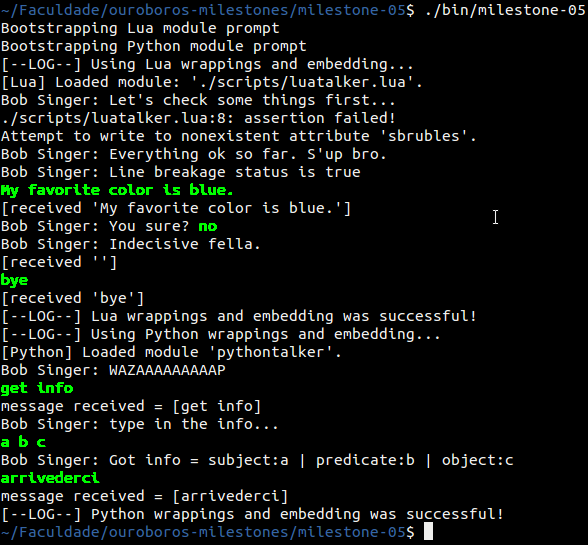
\includegraphics[width=.8\textwidth]{ssMilestone.png}
      \vspace{1em}

      \textit{
        O texto em verde são os comandos enviados pelo usuário.
      }
    \end{center}
  \end{subfigure}
  \label{fig:milestone}
\end{figure}

